\section{Predictive Analysis}
In this section, we consider the problem of predicting the spending behavior of each customer.We will use the main classifier models and evaluate their performances.

First, we will use the customer profile deriving from the K-means clustering, from the previous section.
From the Figure \ref{fig:skmclust}, we recall that we partitioned the dataset in 3 clusters, that represent the \textbf{high-spending} customers, the \textbf{medium-spending} customers and the \textbf{low-spending} customers.
We can see that the clusters are well separated from each other, and so we can use them as customer classification. 

To perform the task, which is a \emph{supervised} one, we split the dataset into training and test set, equal to the 75\% and 25\% of the dataset respectively. Plus, during the splitting, we specify that each partition must have approximately the same relative class frequencies;
that is to manage the unbalance we have in the original dataset, in which the \textbf{medium-spending} $\Leftarrow$ \textbf{DA CONTROLLARE} customers are much more frequent than the other classes.

For each model, we perform a grid search, to find the best values for some hyperparameters; for that, we used a \emph{K-fold cross validation}, with $K=5$.

\subsection{Support Vector Classifier}
\begin{minipage}{0.59\textwidth}
The first model we analyze is the \textbf{SVM}, that is a classifier that searches for an hyperplane that can linearly separate the data points, possibly in a transformed space, in the non-separable case.

We use a Linear Support Vector Classifier and, after the grid search, we found that the best value for the regularization parameter is $C=1000$.\\
With this configuration, we achieved a training accuracy of 0.9906 and a test accuracy of 0.9962.

From the Figure \ref{fig:svm_confusion}, we can see the confusion matrix related to the results on the test set, and we notice that the model made only 4 mistakes on the whole dataset; for that, we have that also the precision and the recall for each class are all above 0.98.
\end{minipage}
\begin{minipage}{0.4\textwidth}
\centering
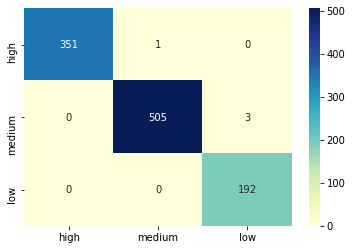
\includegraphics[width=0.90\textwidth]{img/svm_confusion.png}
\captionsetup{justification=centering}
\captionof{figure}{Confusion Matrix\\ for SVM Classifier}
\label{fig:svm_confusion}
\end{minipage}

\subsection{Neural Network}
\begin{minipage}{0.59\textwidth}
Now, we use a Neural Network, in particular a \textbf{Multi Layer Perceptron}.\\
The best values for the hyperparameters that we found was:
\begin{itemize}
\item 1 hidden layer with 50 units
\item Logistic activation function
\item Learning rate equal to 0.001
\item The \emph{lbfgs} optimizer, that can converge faster and with better results on small datasets like ours
\end{itemize}

With this model, we got a training accuracy of 1 and a test accuracy of 0.999; the reason is clear in Figure \ref{fig:nn_confusion}, where we can see that just one data point was misclassified.
\end{minipage}
\begin{minipage}{0.4\textwidth}
\centering
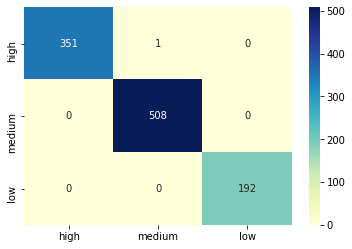
\includegraphics[width=0.90\textwidth]{img/nn_confusion.png}
\captionsetup{justification=centering}
\captionof{figure}{Confusion Matrix\\ for Neural Network}
\label{fig:nn_confusion}
\end{minipage}

\begin{figure}
\centering

\includegraphics[width=\linewidth]{img/decision_tree.png}
\caption{Decision Tree}
\label{fig:decision_tree}
\end{figure}

\subsection{Naive Bayes Classifier}
\begin{minipage}{0.59\textwidth}
\vspace{-13mm}
The Naive Bayes Classifier tries to estimate the class conditional probability for each item, using the \emph{Bayes} theorem, with the assumption that all the features are conditionally independent. In particular, we used a \textbf{GaussianNB}, where the likelihood of the features is assumed to be Gaussian.

In Figure \ref{fig:nb_confusion}, we can see that the performances of this model are slightly worse than the previous ones; in fact, we achieve a training accuracy of 0.9668 and a test accuracy of 0.9525.  
\end{minipage}
\begin{minipage}{0.4\textwidth}
\centering
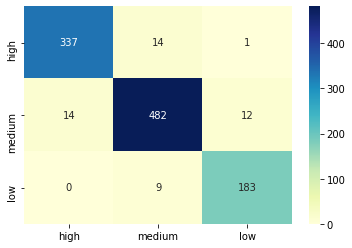
\includegraphics[width=0.90\textwidth]{img/nb_confusion.png}
\captionsetup{justification=centering}
\captionof{figure}{Confusion Matrix\\ for Naive Bayes}
\label{fig:nb_confusion}
\end{minipage}

\subsection{K-Nearest Neighbors}
\begin{minipage}{0.59\textwidth}
The K-Nearest Neighbors model is an instance-based classifier, that, for each record, selects the class label based on the majority of its nearest neighbors.\\
The grid search showed that the best configuration is
\begin{itemize}
\item n\_neighbors equal to 50
\item \emph{distance} as weight function; that makes the weight of a point to be inversely proportional to its distance
\end{itemize}

With these values, we have a training accuracy of 1 and a test accuracy of 0.9781.
The Figure \ref{fig:knn_confusion} shows that some points are misclassified, with some customers, belonging to the high and low profile, incorrectly labeled as medium.
\end{minipage}
\begin{minipage}{0.4\textwidth}
\centering
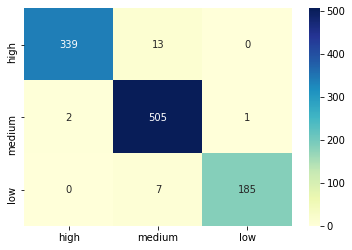
\includegraphics[width=0.90\textwidth]{img/knn_confusion.png}
\captionsetup{justification=centering}
\captionof{figure}{Confusion Matrix\\ for K-Nearest Neighbors}
\label{fig:knn_confusion}
\end{minipage}

\subsection{Decision Tree}
\begin{minipage}{0.59\textwidth}
A Decision Tree model learns some decision rules from the training data, in order to grow a tree that is able to predict the class label for our test points. 
The best configuration found is:
\begin{itemize}
\item \emph{criterion} equal to \emph{gini}
\item \emph{max\_depth} equal to 200
\item \emph{max\_features} equal to 5
\item \emph{min\_samples\_leaf} equal to 1
\item \emph{min\_samples\_split} equal to 2
\item \emph{splitter} equal to \emph{best}
\end{itemize}

The best result is a training accuracy of 1 and a test accuracy of 0.9392, but one of the advantages of this kind of model is that it is easy to interpret, since it can be visualized.
In Figure \ref{fig:decision_tree}, we can have a representation of the best estimator that we found.

The Figure \ref{fig:dt_confusion} shows the model makes several mistakes, with respect to the other classifiers, given that the decision tree is a quite simple model.
\end{minipage}
\begin{minipage}{0.4\textwidth}
\centering
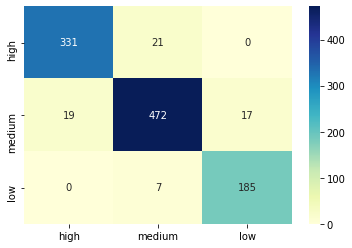
\includegraphics[width=0.90\textwidth]{img/dt_confusion.png}
\captionsetup{justification=centering}
\captionof{figure}{Confusion Matrix\\ for Decision Tree}
\label{fig:dt_confusion}
\end{minipage}

\subsection{Random Forest}
\begin{minipage}{0.59\textwidth}
Lastly, we analyze the Random Forest. It is an \emph{ensemble} model, composed by several decision trees, and the result is given by averaging the predictions of the single classifier.
In this case, the best hyperparameters are:
\begin{itemize}
\item \emph{max\_depth} equal to 30
\item \emph{max\_features} equal to 1
\item \emph{min\_samples\_leaf} equal to 1
\item \emph{min\_samples\_split} equal to 2
\item \emph{n\_estimators} equal to 1500
\end{itemize}
As a results, we have a training accuracy of 1 and a test accuracy of 0.9952; these good results are confirmed by the Figure \ref{fig:rf_confusion.png}, that shows that the errors made by the model are very few.
\end{minipage}
\begin{minipage}{0.4\textwidth}
\centering
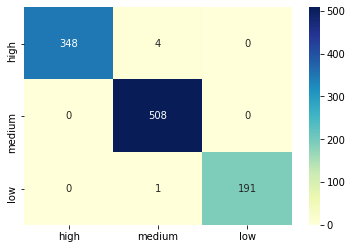
\includegraphics[width=0.90\textwidth]{img/rf_confusion.png}
\captionsetup{justification=centering}
\captionof{figure}{Confusion Matrix\\ for Random Forest}
\label{fig:rf_confusion}
\end{minipage}
